\documentclass{article}
\usepackage{amsmath}
\usepackage{graphicx}

\begin{document}

\section*{Figuring out what happens with the solver
  \centering when there is attenuation}

I like to use simple test cases because they clarify to me what is
\textit{not} the problem. So I will be considering the following
situation: a $1\times 1\times 1$ meter box, and I will be evaluating
the solution at the center of that cube. The left face of the cube is
marked as a port, as is the right. So the equations we will be
solving when we are driving the left port are:
\begin{align*}
  -\omega^2 p(x,y,z) - c^2 \Delta p(x,y,z) &= 0, \\
  p(x=0,y,z) &= 1, && \text{(left boundary)}\\
  p(x=1,y,z) &= 0, && \text{(right boundary)} \\
    \frac{\partial p}{\partial n} &= 0,
     && \text{(all other boundaries)}
\end{align*}
The wave speed is computed as
\begin{align*}
  c = \sqrt{\frac{K}{\rho}},
\end{align*}
where $K$ is the bulk modulus and $\rho$ is the density, both of which
are read from the input file as frequency-dependent quantities, and
which can both be complex-valued.


\section{Testing the pressure}

The set-up is chosen so that the solution is one-dimensional. As a
consequence, the solution only depends on $x$ and we can easily derive
it as
\begin{align*}
  p(x,y,z) = p(x) &= \frac{e^{jkx} - e^{-jk(2L-x)}}{1 - e^{-2jkL}},
\end{align*}
with $L=1$ and $k=\frac{\omega}{c}$. It is not difficult to verify
that indeed the boundary conditions are satisfied:
\begin{align*}
  p(0) &= \frac{e^{jk0} - e^{-jk(2L-0)}}{1 - e^{-2jkL}}
  =
  \frac{1 - e^{-2jkL}}{1 - e^{-2jkL}} = 1,
  \\
  p(L) &= \frac{e^{jkL} - e^{-jk(2L-L)}}{1 - e^{-2jkL}}
  = \frac{e^{jkL} - e^{-jkL}}{1 - e^{-2jkL}} = 0.
\end{align*}
It is also not difficult to check that the equation itself is
satisfied:
\begin{align*}
  -\omega^2 p(x) - c^2 \Delta p(x)
  &= -\omega^2 p(x) - c^2 p''(x)\\
  &= -\omega^2 p(x) - c^2 (jk)^2 p''(x)  \\
  &= (k^2c^2-\omega^2) p(x) \\
  &= \left(\frac{\omega^2}{c^2}c^2-\omega^2\right) p(x)\\
  &= 0.
\end{align*}

With this solution, evaluated at the center of the box of length
$L=1$, we obtain
\begin{align*}
  p_\text{center} &= p(0.5)
  \\
  &= \frac{e^{\frac{jk}{2}} - e^{-\frac{3jk}{2}}}{1 - e^{-2jk}}
  \\
  &= \frac{e^{\frac{jk}{2}} - e^{-\frac{3jk}{2}}}{e^{jk} - e^{-jk}}
  \\
  &= \frac{e^{\frac{j\omega}{2c}} - e^{-\frac{3j\omega}{2c}}}{1 - e^{-\frac{2j\omega}{c}}}
  \\
  &= \frac{e^{\frac{j\omega}{2}\sqrt{\frac{\rho}{K}}} - e^{-\frac{3j\omega}{2}\sqrt{\frac{\rho}{K}}}}{1 - e^{-2j\omega\sqrt{\frac{\rho}{K}}}}
\end{align*}
We will consider this expression for two special cases below, without
and with attenuation.


\subsection{No attenuation}

Let us consider the evaluation of the pressure at the center of the
box for the special case without attenuation. For simplicity, we
choose $\rho=K=1$ and consequently $c=1$ and $k=\omega$. Then, based
on the formulas in the \texttt{readme.md} file at the top level of the
github repository, we have
\begin{align*}
  p(x)
  &=
  \frac{e^{jkx} - e^{-jk(2L-x)}}{1 - e^{-2jkL}}.
\end{align*}
This formula, after a good bit of massaging, can be restated as
follows for real-valued $k$:
\begin{align*}
  p(x)
  &=
  \frac{\sin(k(L-x))}{\sin(kL)}.
  \\
  &=
  \frac{\sin(\omega(1-x))}{\sin(\omega)}.
\end{align*}
This expression, unsurprisingly, has singularities for
$\omega=\pi,2\pi,3\pi,...$, where the cavity is in resonance. This
corresponds to frequencies $f=0.5, 1, 1.5, \ldots$ Hertz. As a
consequence, we better consider frequences below the first resonance,
i.e., $\omega<\pi$, i.e., $f<0.5$ Hertz.

That said, for the specific case of the center of the box (at $x=0.5$), we get
\begin{align*}
  p_\text{center}
  &= 
  \frac{\sin(\omega/2)}{\sin(\omega)}.
\end{align*}
In the low-frequency case, $\omega\ll 1$, we have the asymptotic
behavior $\sin(t)\approx t$ and so
\begin{align*}
  p_\text{center}
  &\approx
  \frac{\omega/2}{\omega}
  = \frac 12.
\end{align*}
This makes sense: In the low-frequency limit, the length of the cavity
is much less than the wavelength and so the pressure simply decreases
linearly from one at the left end to zero at the right end -- implying
a pressure of 0.5 at the center of the object.

We can plot what the program produces for a number of frequencies in
the range between 0.01 and 1 Hz:
%
% dii_frequency_response.csv, columns 1 (frequency), 14 (real part of
% pressure), 15 (imaginary part of pressure)
%

\begin{center}
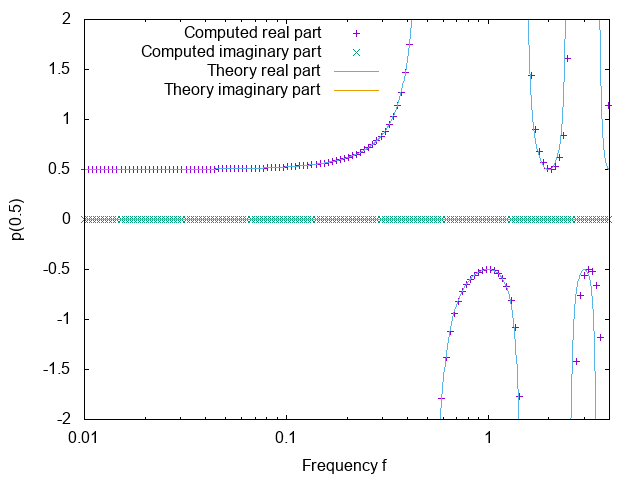
\includegraphics[width=0.7\textwidth]{unit-cube/no-attenuation/pressure-at-center.png}
\end{center}

As can be seen, the computations (shown as the purple and green crosses)
are an excellent match for the expected theoretical behavior, at least
in the low-frequency regime. Furthermore, the singularity (resonance)
is at $f=0.5$ Hz, again as expected. (For higher frequencies, the
crosses are no longer a good fit, but this is because we compute on a
mesh that has only $16\times 16\times 16$ cells. We can not expect it to
accurately resolve the solution for frequencies $f\ge 4$ where the
wavelength $\lambda=c/f$ drops below four cell diameters.)


\subsection{With attenuation}

Let us now consider the case with attenuation. Specifically, we will
choose the same box of length $L=1$, but use $\rho=1-j, K=1$ and
consequently $c=\sqrt{\frac{K}{\rho}}=\sqrt{\frac{1}{1-j}}=\frac{1}{2^{1/4}}e^{j\pi/8}$ 
and $k=\omega/c=2^{1/4}e^{-j\pi/8} \omega$. Then, again based
on the formulas in the \texttt{readme.md} file at the top level of the
github repository, we have
\begin{align*}
  p(x)
  &=
  \frac{e^{jk(L-x)} - e^{-jk(L-x)}}{e^{jkL} - e^{-jkL}}.
\end{align*}
This time, because $k$ is not real valued, we cannot replace $e^{ja}$
by $\cos(a)+j\sin(a)$, and instead need to use the expression as
is. We can, however, simplify it to
\begin{align*}
  p(x)
  &=
  \frac{\sinh(jk(L-x))}{\sinh(jkL)}.
\end{align*}
Consequently,
\begin{align*}
  p_\text{center}
  &=
  \frac{\sinh(jk/2))}{\sinh(jk)}.
\end{align*}
We can again make the same observation that in the low-frequency
limit, $\sinh(t)=\frac 12(e^t-e^{-t})\approx \frac 12[(1+t)-(1-t)]=t$,
and so
\begin{align*}
  p_\text{center}
  &=
  \frac{\sinh(jk/2))}{\sinh(jk)}
  \approx
  \frac{jk/2}{jk}
  = \frac 12.
\end{align*}
The reasoning for this is as before: With or without damping, in the
low-frequency regime, the pressure is linear and so equal to one half
at the center of the domain.

We can again output the results of our computations:
\begin{center}
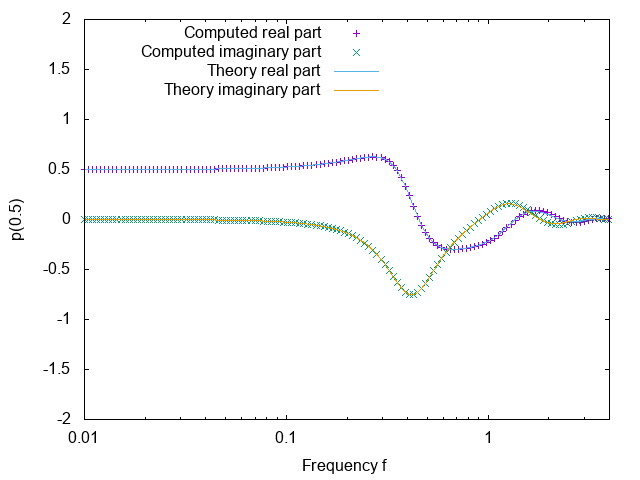
\includegraphics[width=0.7\textwidth]{unit-cube/with-attenuation/pressure-at-center.png}
\end{center}
As before, the results provide an excellent match to the theoretical expectations.


\section{Testing the velocity}

We can also look at the velocity at the center point. The velocity is
defined as $\mathbf u(\mathbf x)=j\omega \nabla p(\mathbf x)$ but
because everything only depends on the $x$ coordinate, only one
component of the velocity is nonzero and we can simply denote it by
(non-bold) $u(x)=-\frac{1}{j\rho\omega}\frac{d}{dx} p(x)$.

\subsection{No attenuation}

With the expression for the pressure above for the case without
attenuation, we get
\begin{align*}
  u(x)
  &=
  -\frac{1}{j\rho\omega} \frac{d}{dx} \frac{\sin(\omega(1-x))}{\sin(\omega)}
  \\
  &=
  -\frac{1}{j\rho} \frac{-\cos(\omega(1-x))}{\sin(\omega)},
\end{align*}
and consequently
\begin{align*}
  u_\text{center}
  &=
  \frac{1}{j\rho} \frac{\cos(\omega/2)}{\sin(\omega)}
  \\
  &=
  -\frac{j}{\rho} \frac{\cos(\omega/2)}{\sin(\omega)}.
\end{align*}
In the low-frequency regime, this expression has the asymptotic behavior
\begin{align*}
  u_\text{center}
  &\approx
  -\frac{j}{\rho} \frac{1}{\omega}.
\end{align*}


We can again compare this against what the program computes:
\begin{center}
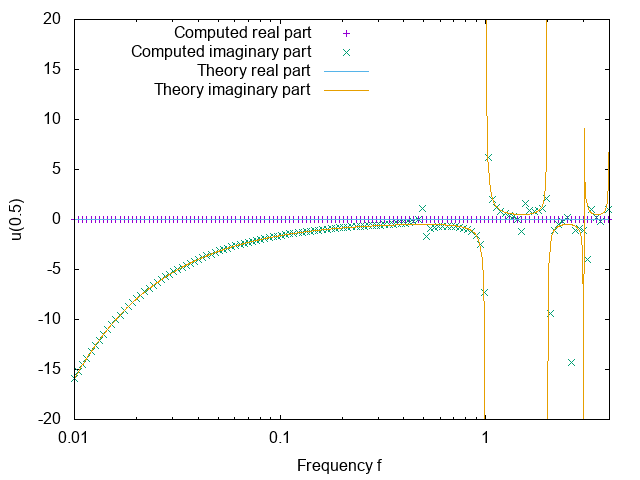
\includegraphics[width=0.7\textwidth]{unit-cube/no-attenuation/velocity-at-center.png}
\end{center}
As before, in the low-frequency range, the agreement is
excellent. (And, as before, the agreement is not good in the
high-frequency range because the mesh is too coarse. There is also a
little blip at the first resonance at $f=0.5$ Hz. This is because
while the pressure becomes very large at the resonance, the
\textit{exact} velocity stays bounded -- but the numerical
approximation becomes poor.)

While not shown
in the figure, one can easily check that the asymptotic behavior
outlined above is also respected by the actual computed data points.



\subsection{With attenuation}

For the case with attenuation, let us start with
\begin{align*}
  p(x)
  &=
  \frac{\sinh(jk(L-x))}{\sinh(jkL)},
\end{align*}
to compute
\begin{align*}
  u(x)
  &=
  -\frac{1}{j\rho\omega} \frac{d}{dx}
  \frac{\sinh(jk(L-x))}{\sinh(jkL)}
  \\
  &=
  -\frac{1}{j\rho\omega}
  \frac{-jk\cosh(jk(L-x))}{\sinh(jkL)}
  \\
  &=
  \frac{k}{\rho\omega}
  \frac{\cosh(jk(L-x))}{\sinh(jkL)}
  \\
  &=
  \frac{1}{\rho c}
  \frac{\cosh(jk(L-x))}{\sinh(jkL)}
  \\
  &=
  \frac{1}{\rho}\sqrt{\frac{\rho}{K}}
  \frac{\cosh(jk(L-x))}{\sinh(jkL)}
  \\
  &=
  \frac{1}{\sqrt{\rho K}}
  \frac{\cosh(jk(L-x))}{\sinh(jkL)}.
\end{align*}
From this we then get
\begin{align*}
  u_\text{center}
  &=
  \frac{1}{\sqrt{\rho K}}
  \frac{\cosh(jk/2)}{\sinh(jk)}.
\end{align*}
In the low-frequency regime, the asymptotic expansion of this
expression is
\begin{align*}
  u_\text{center}
  &\approx
  \frac{1}{\sqrt{\rho K}}
  \frac{1}{jk}
  =
  -\frac{j}{\sqrt{\rho K}}
  \frac{\sqrt{K}}{\omega\sqrt{\rho}}
  =
  -\frac{j}{\omega\rho}.
\end{align*}
This is the same expression as for the case without attenuation,
except that now $\rho$ may be complex-valued.

If we compare the exact expression against computations, we obtain the
following figure:
\begin{center}
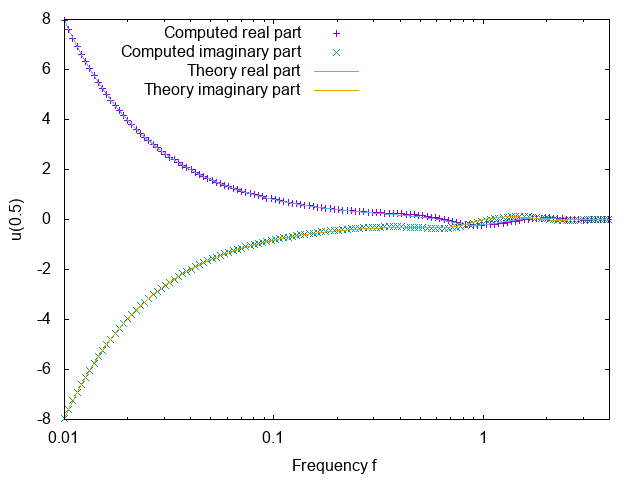
\includegraphics[width=0.7\textwidth]{unit-cube/with-attenuation/velocity-at-center.png}
\end{center}
The match is again excellent.


\section{On a small, rectangular wave guide}

The original report of results that deviate from those that are
expected were for a small rectangular wave guide of size 5mm by 5mm by
10mm. We can adapt the case above to the same situation
here. Specifically,the solution in general is given by
\begin{align*}
  p(x)
  &=
  \frac{\sinh(jk(L-x))}{\sinh(jkL)},
  \\
  u(x)
  &=
  \frac{1}{\sqrt{\rho K}}
  \frac{\cosh(jk(L-x))}{\sinh(jkL)}.
\end{align*}
We set $L=0.01$ (10mm), and recall
$k=\frac{\omega}{c}=\sqrt{\frac{\rho}{K}}\omega$. Since the domain is
smaller by a factor of 100, we increase the frequency range for which
we compute the cavity's response by a factor of 100. We will evaluate
the solution at the point $x=L/2$ as before.

As the results in the following two sub-sections show, computational
results are again very close to those obtain through theory, at least
in that part of the frequency range where the mesh resolves the wave length.

\subsection{No attenuation}

We can again compute the response with the solver and compare it
against the predictions of the formulas above. We again use
$K=1,\rho=1$ as material parameters.

\begin{center}
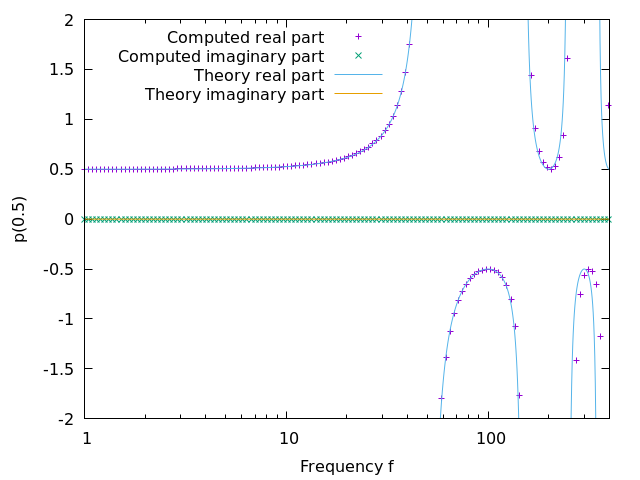
\includegraphics[width=0.48\textwidth]{wave-guide/no-attenuation/pressure-at-center.png}
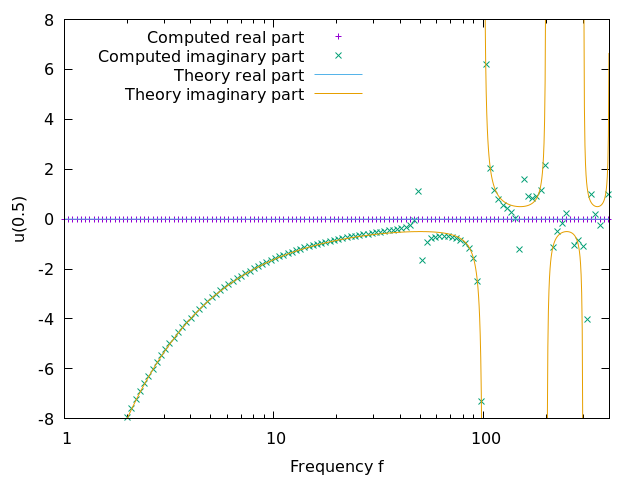
\includegraphics[width=0.48\textwidth]{wave-guide/no-attenuation/velocity-at-center.png}
\end{center}

These results again track very well with theoretical predictions.

\subsection{With attenuation}

Setting instead $K=1,\rho=1-j$, we obtain the following figures that
again show excellent match between theory and computation:

\begin{center}
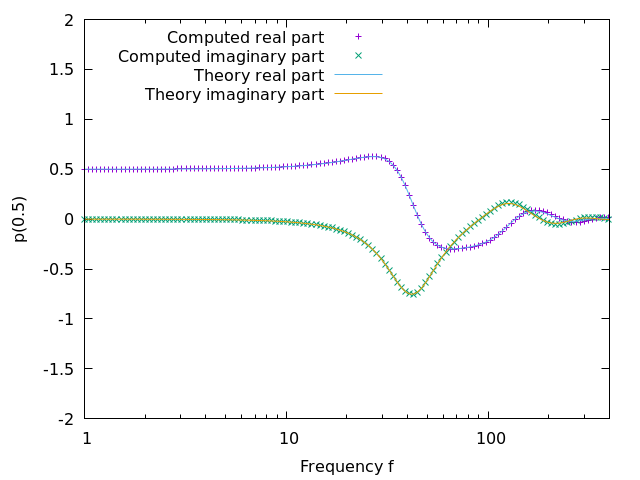
\includegraphics[width=0.48\textwidth]{wave-guide/with-attenuation/pressure-at-center.png}
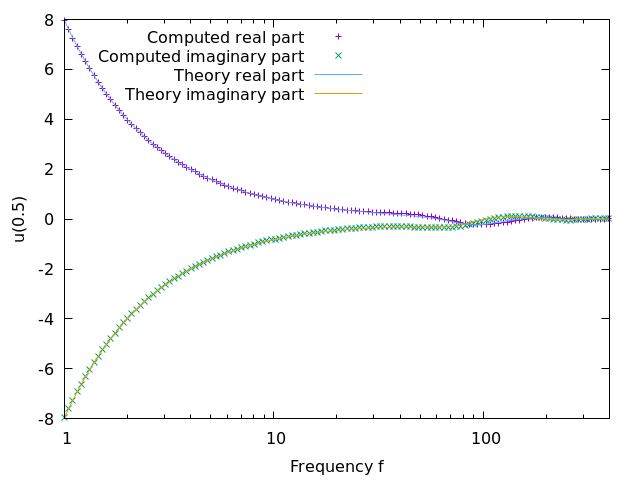
\includegraphics[width=0.48\textwidth]{wave-guide/with-attenuation/velocity-at-center.png}
\end{center}



\section{Using a tetrahedral mesh for the small, rectangular wave guide}

Another observation was that the mismatch between theory and
computation appeared on a generated mesh that used tetrahedra. On the
other hand, all of the computations above have used hexahedral meshes.

To test whether this has any effects on the computational results, I
re-ran the tests of the previous section on a mesh that subdivides the
small rectangular wave guide into tetrahedra. This is done by
subdividing the hexahdedra used previously into 24
tetrahedra, and this results in cells with a substantially smaller
size than the hexahedra used before -- for which one could expect
higher accuracy than what was available before. As a consequence, for
the experiments shown in this section, we start with a $8\times
8\times 8$ hexahedral mesh instead, which after subdivision into
tetrahedra is comparable in mesh size to the  $16\times 16\times 16$
mesh used whenceforth.

The results are shown below and illustrate that we again get excellent
agreement, regardless of whether we use hexahedra or tetrahedra.

\subsection{No attenuation}

We can again compute the response with the solver and compare it
against the predictions of the formulas above. We again use
$K=1,\rho=1$ as material parameters.

\begin{center}
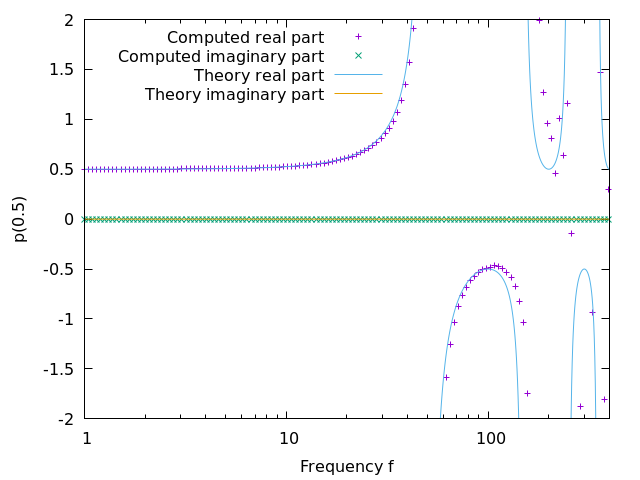
\includegraphics[width=0.48\textwidth]{wave-guide-tet/no-attenuation/pressure-at-center.png}
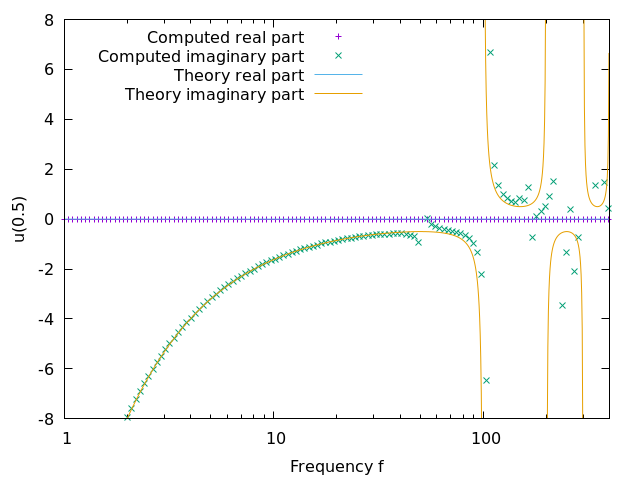
\includegraphics[width=0.48\textwidth]{wave-guide-tet/no-attenuation/velocity-at-center.png}
\end{center}

These results again track very well with theoretical predictions.

\subsection{With attenuation}

Setting instead $K=1,\rho=1-j$, we obtain the following figures that
again show excellent match between theory and computation:

\begin{center}
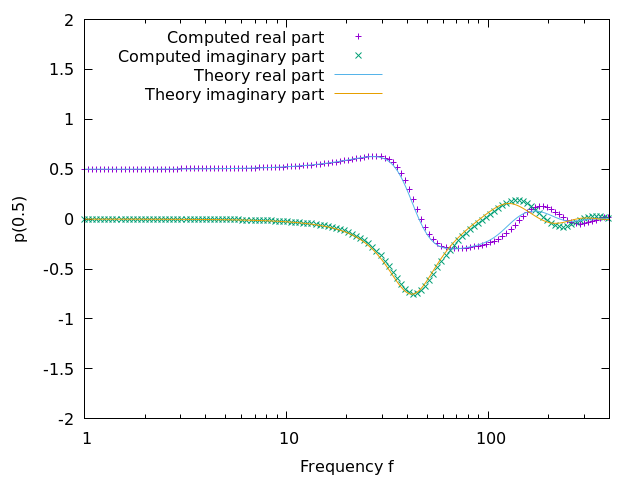
\includegraphics[width=0.48\textwidth]{wave-guide-tet/with-attenuation/pressure-at-center.png}
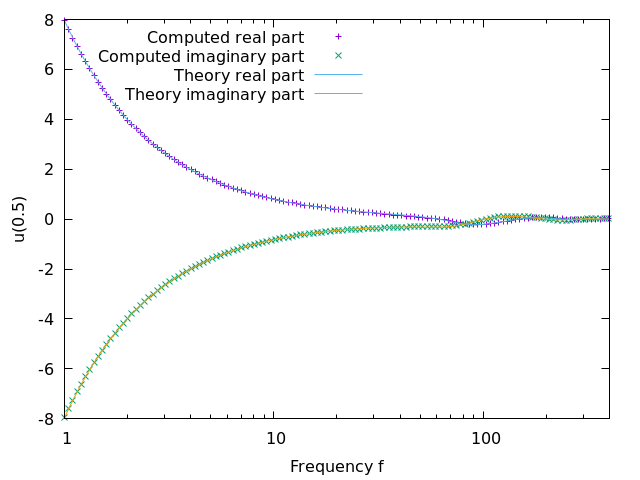
\includegraphics[width=0.48\textwidth]{wave-guide-tet/with-attenuation/velocity-at-center.png}
\end{center}


\section{Testing with realistic material properties}

To further narrow the gap between the simulations above and those from
Jason's cases, I set material properties to $\rho=1.43257-8.72485j$
and $K=101582+2796.01j$, which leads to a wave speed of
$c=\sqrt{\frac{\rho}{K}}=\sqrt{\frac{1.43257-8.72485j}{101582+2796.01j}}=(80.76+70.51j)$m/s. With
$L=0.01$m, this leads to a first resonance at $f=Re(c/L)\approx 8075$
Hz (though this resonance is heavily damped, given the material
parameters). So we will be considering a frequency range between 10
and 10,000 Hz.

Using again the same exact solution from above, but with the altered
material properties, we obtain the following pictures:
\begin{center}
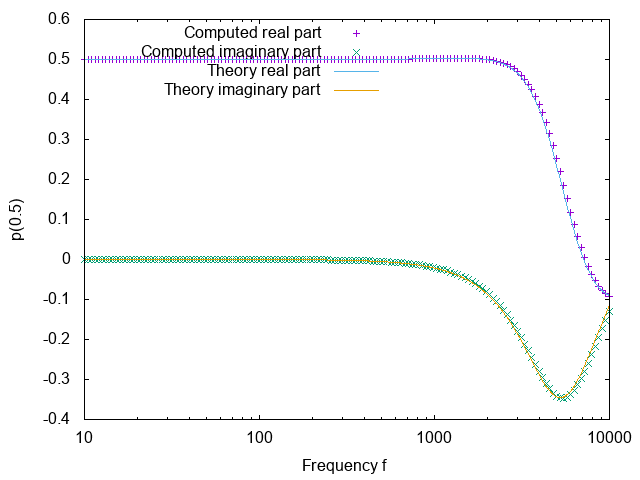
\includegraphics[width=0.48\textwidth]{wave-guide-tet-real-material/pressure-at-center.png}
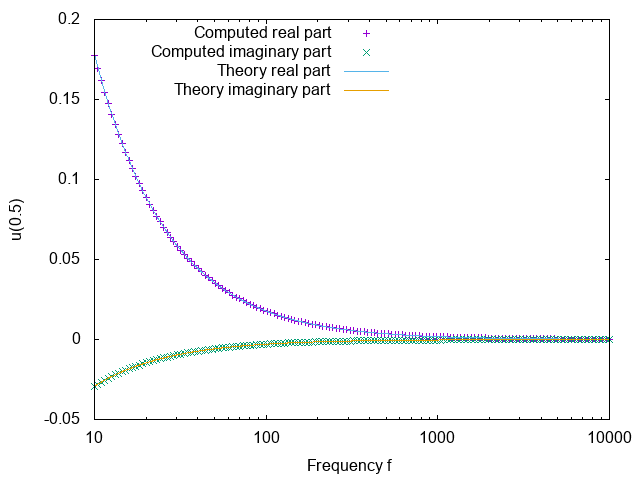
\includegraphics[width=0.48\textwidth]{wave-guide-tet-real-material/velocity-at-center.png}
\end{center}
Again, the computed results are essentially indistinguishable to the
theoretical predictions.

One may ask whether the error between the computed solution and theory
is noticeable but simply not visible because of the scale of these
graphs. To test this, the following two figures show the relative
error, computed as the absolute values of the real and imaginary parts
of the quantities
\begin{align*}
  \frac{p_\text{computed} - p_\text{theory}}{|p_\text{theory}|},
  \qquad\qquad
  \frac{u_\text{computed} - u_\text{theory}}{|u_\text{theory}|}.
\end{align*}
\begin{center}
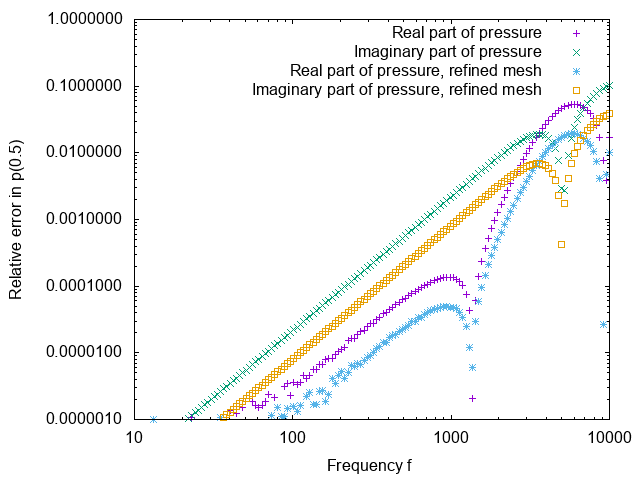
\includegraphics[width=0.48\textwidth]{wave-guide-tet-real-material/error-pressure-at-center.png}
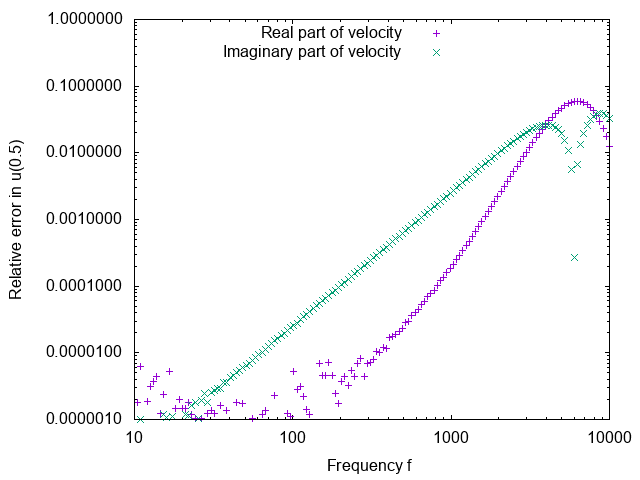
\includegraphics[width=0.48\textwidth]{wave-guide-tet-real-material/error-velocity-at-center.png}
\end{center}

These figures show that not only do the computed solutions lie on top
of the theoretical predictions, but in fact the difference is also
quite small even on this relatively coarse mesh: Pressure errors are
generally less than a few percent when close to the first resonance
(and much smaller for lower frequencies), and the
same is true for the velocity. It is worth noting that the mesh is so
coarse that we no longer adequately resolve the solution at the first
resonance.

To illustrate that we can obtain better results on finer meshes, the
figures above also show the same error metrics for a mesh that is once
more refined. The data show that the error in the pressure is reduced
by a factor of 4 with mesh refinement, and by a factor of 2 for the
velocity. This is in perfect accordance with the predictions from
numerical analysis.


\section{Testing with the original mesh}

The mesh used so far was built within the solver, for the geometry at
hand. The next check is to use the mesh provided by Jason, originally
generated by gmsh. This required a small amount of adaptation because
its long axis is the $z$ axis, rather than $x$ axis used before, and
the mesh uses a scaling factor of 0.001 (that is, the mesh has size
$0.5\times 0.5\times 1$ and is scaled down by a factor of 1000 to
arrive at units in meters).

With this mesh, and with the material properties as above (the first
line of the \texttt{materials.txt} file used by Jason's test case),
the results look as follows (for the mesh as read from file, as well
as a once-refined version):
\begin{center}
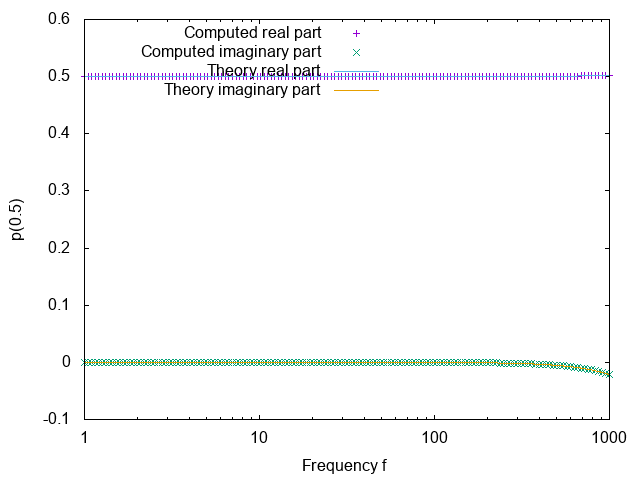
\includegraphics[width=0.48\textwidth]{wave-guide-tet-real-material-jasons-mesh-0/pressure-at-center.png}
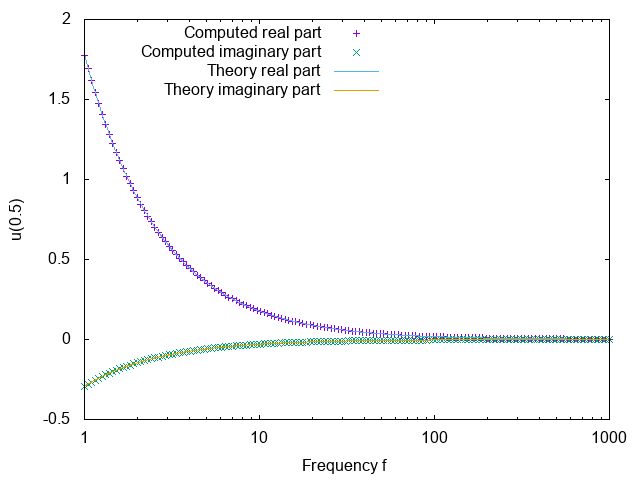
\includegraphics[width=0.48\textwidth]{wave-guide-tet-real-material-jasons-mesh-0/velocity-at-center.png}
\end{center}

We can again compute the errors and notice that they are even better
than with the mesh internally created:
\begin{center}
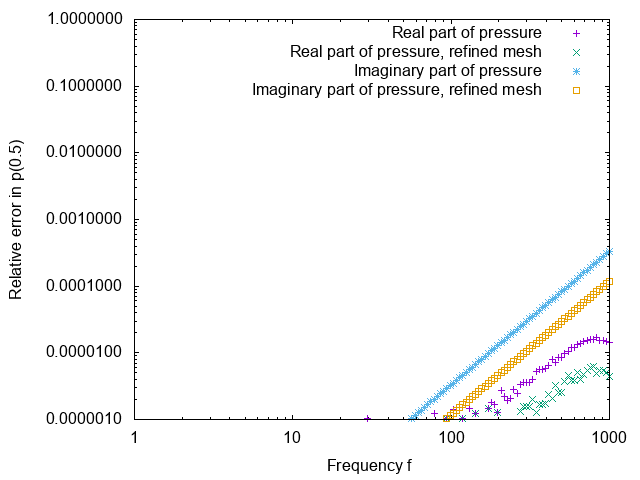
\includegraphics[width=0.48\textwidth]{wave-guide-tet-real-material-jasons-mesh-0/error-pressure-at-center.png}
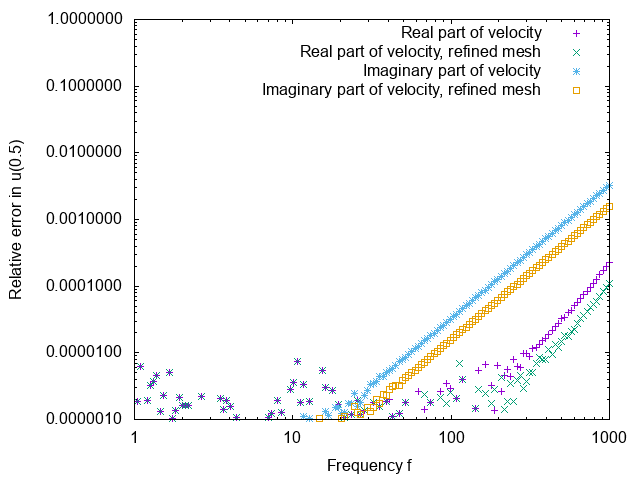
\includegraphics[width=0.48\textwidth]{wave-guide-tet-real-material-jasons-mesh-0/error-velocity-at-center.png}
\end{center}

In the testcase Jason sent me, computations are done with quadratic
finite elements. We can repeat the same graphics for these as well;
the solution values look like the ones above, but it is interesting to
see the errors on the same scale as above -- showing that the error is
more than an order of magnitude smaller when using quadratic elements than
with the linear elements used before:
\begin{center}
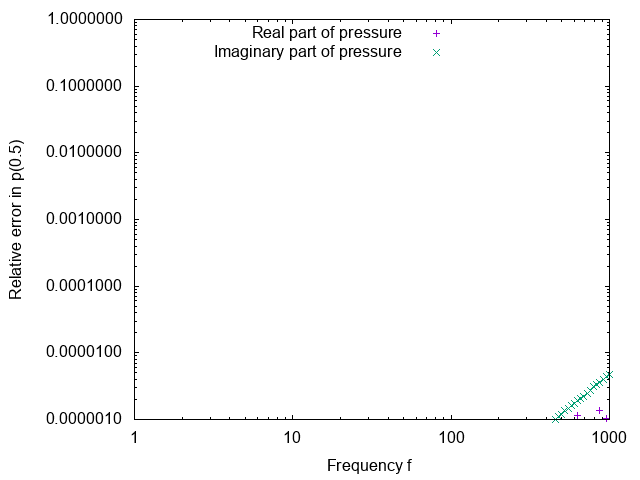
\includegraphics[width=0.48\textwidth]{wave-guide-tet-real-material-jasons-mesh-0-quadratic/error-pressure-at-center.png}
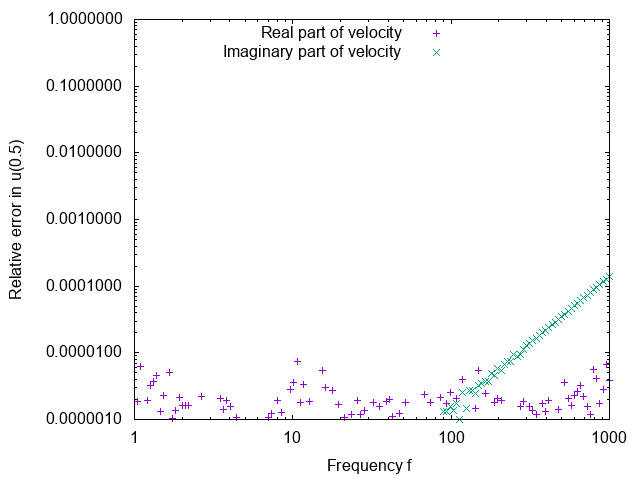
\includegraphics[width=0.48\textwidth]{wave-guide-tet-real-material-jasons-mesh-0-quadratic/error-velocity-at-center.png}
\end{center}


\section{Testing the impedance computations}

The tests above all checked that the solution is computed correctly
(which it apparently is, based on all of the results shown). From the
solution, the solver then computes pressures and velocities at the
``ports'' of the geometry, which are then further used to compute
impedances. So let us consider these port pressures and velocities.

The situation considered here is about a geometry where we prescribe
the pressure at individual ports to either be zero or one, and that is
reflected in the analytic expression for the pressure,
\begin{align*}
  p(x)
  &=
  \frac{\sinh(jk(L-x))}{\sinh(jkL)},
\end{align*}
which is either one at $x=0$ and zero at $x=L$. The velocity is given by
\begin{align*}
  u(x)
  &=
  \frac{1}{\sqrt{\rho K}}
  \frac{\cosh(jk(L-x))}{\sinh(jkL)},
\end{align*}
and this evaluates to
\begin{align*}
  u(0)
  &=
  \frac{1}{\sqrt{\rho K}}
  \frac{\cosh(jkL)}{\sinh(jkL)}
  =
  \frac{1}{\sqrt{\rho K}\tanh(jkL)},
\\
  u(L)
  &=
  \frac{1}{\sqrt{\rho K}}
  \frac{\cosh(0))}{\sinh(jkL)}
  =
  \frac{1}{\sqrt{\rho K}\sinh(jkL)}.
\end{align*}

The impedance is defined as 
\begin{align*}
  Z = \frac{p(0)}{u(0)},
\end{align*}
where $p$ is the pressure applied to a port (which is equal to one in
our case), and $u$ is the corresponding volumetric velocity at that
port, averaged over the entire port. For the given situation, at
$x=0$, this corresponds to
\begin{align*}
  Z = \frac{p(0)}{u(0)} 
  = 
  \frac{1}
  {\frac{1}{\sqrt{\rho K}}
  \frac{\cosh(jkL)}{\sinh(jkL)}}
  = 
  \sqrt{\rho K}\tanh(jkL),
\end{align*}
where as before $k=\frac{\omega}{c}=\sqrt{\frac{\rho}{K}}\omega$.

The following figure shows the impedance so calculated analytically,
and compares it to the values computed from the velocity output at the
port by the program.
\begin{center}
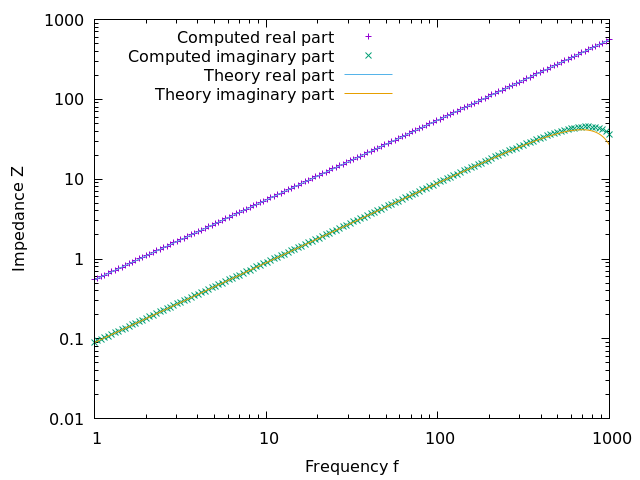
\includegraphics[width=0.48\textwidth]{wave-guide-tet-real-material-jasons-mesh-0/impedance.png}
\end{center}
As maybe expected by now, these match well.

In Jason's presentations, there are also trend lines for low-frequency
limits. To this end, we can note that for the impedance $Z$, we can
estimate as follows in the limit of small $\omega$:
\begin{align*}
  Z
  &= 
  \sqrt{\rho K}\tanh(\xi)
  \\
  &= 
  \sqrt{\rho K}
  \frac{\sinh(\xi)}
       {\cosh(\xi)}
  \\
  &= 
  \sqrt{\rho K}
  \frac{e^\xi - e^{-\xi}}
       {e^\xi + e^{-\xi}}
  \\
  &\approx
  \sqrt{\rho K}
  \frac{(1+\xi) - (1-\xi)}
       {(1+\xi) + (1-\xi)}
  \\ 
  &=
  \sqrt{\rho K}
  \frac{2\xi}
       {2}
  \\
  &=
  \sqrt{\rho K} \xi,
\end{align*}
where $\xi=j\sqrt{\frac{\rho}{K}}\omega L$. Substituting $\xi$ back
into the equation above yields, for the low-frequency limit:
\begin{align*}
  Z
  &\approx
  \sqrt{\rho K} \times j\sqrt{\frac{\rho}{K}}\omega L
  \\
  &=
  j \rho L \omega.
\end{align*}
This formula matches the one in Jason't \texttt{readme.txt} file in a
recent zip file, with the exception that there it divides by $S$ (the
surface area of the port).

For the material parameters used for the computations shown above, 
$\rho=1.43257-8.72485*i$, and so at the leftmost point in the figure
($f=1,\omega=2\pi$), we would obtain an impedance of $Z=
(1.43257j+8.72485) \times 0.01 \times 2\pi$, that is: 
$Z=0.548+0.09001j$. This also matches the values one can read from the
figure above.


\end{document}
